% Chapter 2

\chapter{Related Work} % Write in your own chapter title
\label{Chapter2}
\lhead{Chapter 2. \emph{Related Work}} % Write in your own chapter title to set the page header

The study of \glspl{uav} is wide and goes

In this chapter, we introduce a state of the art on \glspl{ums}, focusing on their main features, objectives, complexity and accessibility.

\section{UAV Simulators}
%Hablar de todo tipo de simuladores (Comerciales, no comerciales...)
Computer simulations, and their extension into videogames, of \glspl{us} are an emerging topic. There are at least three motivations for these type of simulators. One is the role of simulators in adoption of new technology, another is their potential for low cost training, and finally their utility in research. The four critera used to jugde the quality of any virtual simulator are defined in \cite{alexander2005gaming}:
\begin{enumerate}
\item \emph{Physical Fidelity}: It can be described as the extent to which the virtual environment emulates the real world. A simulator with high physical fidelity is able to render the environment with high resolution textures, shaders, lighting, reflection, and bump mapping. A low physical fidelity simulator uses 2D rendering and no sound is required.

\item \emph{Functional Fidelity}: The degree to which the simulation acts like the operational equipment in reacting to the tasks executed by the trainee. High functional fidelity is defined as the simulation of most of the forces acting on a vehicle and its actuators including gravity, drag, and accelerations from motors and collisions on specific elements of the vehicle. A low functional fidelity simulator does not simulate forces applied to the vehicle but only velocities or absolute position.

\item \emph{Ease of Development}: It is defined by how easy/difficult the simulator can be modified, and the available documentation from the author.

\item \emph{Cost}: For a simulator to be useful it must not be time consuming to install or run and accessible in terms of initial monetary cost for both the developer and end user. The simulator developed in this work is focused on maximizing this criteria.
\end{enumerate}

%Talk about the low cost UV simulators surveyed in craighead2007survey
\cite{craighead2007survey} surveys multiple \gls{us} simulators, both commercial and open-source, and provides a subjective rating of capabilities in terms of physical fidelity, functional fidelity, ease of use, and cost. For the purposes of this work, we focus only on those rated as "Low" in the Cost criteria. Table \ref{table:lowCostUVSimulators} summarizes the rating results of the aforementioned "Low cost" \gls{us} Simulators:

\begin{itemize}
\item \emph{FlightGear}: FlightGear \cite{flightGear} is a 3D open source simulator, very realistic and focused on simulating the flight of a single aircraft vehicle. It is available as a free download under GPL license. The entire source code is available for modification and is under constant development. The application runs on Windows, Mac, and Linux operating systems. It has been used for various academic projects. For example, Summers, et al. in \cite{summers2002determination} used FlightGear to simulate a \gls{uav} carrying environmental sensors and Cervin, et al. in \cite{cervin20043d} used FlightGear to create an interface for a real \gls{uav}.

\item \emph{Simbad}: Simbad \cite{simbad} is a Java 3d robot simulator for scientific and educational purposes. It is mainly dedicated to researchers/programmers who want a simple basis for studying Situated Artificial Intelligence, Machine Learning, and more generally AI algorithms, in the context of Autonomous Robotics and Autonomous Agents. It is not intended to provide a real world simulation and is kept voluntarily readable and simple.

\item \emph{SimRobot}: SimRobot \cite{simrobot} is a physics based robot simulator with a 3D OpenGL based display. Several sensor types are supported, including cameras, range sensors, touch 
sensors, and actuator state. It was used by the German team for the 2005 RoboCup competition \cite{laue2006simrobot}.
\end{itemize}

Analyzing the simulators detailed above, it is appreciable that the Functional Fidelity rating for all of them is not high, thus we cannot use them to easily analyze human control over them. Also, none of them focuses on the field of \glspl{uav} purely, but cover general unmanned robots or aircrafts instead. This is because at the time when these simulators were released, \glspl{uav} did not have as much importance as now.

%More recent work (focused on UAVs strictely)
Recently, the rapidly increasing interest in \glspl{uav} has caused that they are no longer part of a flight simulator or a type of robot in a general robot simulator. Small/micro UAVs have become applicable in civilian circumstances like remote sensing, mapping, traffic monitoring, search and rescue, etc. They are expendable, easy to be built and operated. Most of them can be operated by one to two people, or even be hand-carried and hand-launched \cite{roadmap2002roadmap,wu2004micro}. This has caused a large increase in the development of the so-called \emph{Autopilots}.

%Autopilots - Survey
\emph{Autopilots} are systems to guide the \glspl{uav} in flight with no assistance from human operators, consisting of both hardware and its supporting software. In \cite{chao2010autopilots}, both commercial and research autopilot systems for small \glspl{uav} are reviewed and discussed in detail. Since this work is not emphasized on hardware, the most remarkable autopilot from that survey, in terms of software development, is \emph{Paparazzi}.

%Paparazzi
Paparazzi \cite{brisset2006paparazzi} is an open-source project, very popular among researchers, highlighted by offering good flexibility and ease to modify the autopilot based on own requirements (High "Ease of development" rate, following the criteria of \cite{alexander2005gaming}). For the software, it can achieve waypoint tracking, auto-takeoff and landing, and altitude hold. Figure \ref{fig:paparazziGCS} shows how this software tries to imitate a real \gls{gcs}. A disadvantage of Paparazzi (and more generally, of all autopilots surveyed in \cite{chao2010autopilots}), is the lack of support for cooperative control functions, required for some large area tasks that need multiple \glspl{uav} to perform them.

\begin{figure}[hbt]
	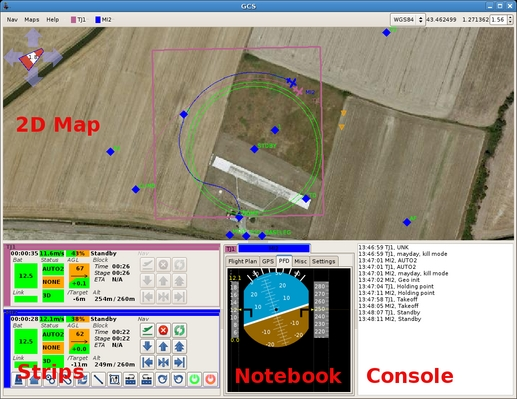
\includegraphics[width=\textwidth]{./Figures/PaparazziGCS.jpg}
	\centering
	\caption{Paparazzi GCS. The Paparazzi Ground Control Station is the heart of the system and the user's primary interaction interface.}
	\label{fig:paparazziGCS}
\end{figure}

%Multi UAV simulators and autopilots
The increasing demand and complexity of \gls{uav} applications has brought into focus several challenges associated with multiple \glspl{uav} \cite{bertuccelli2009real}. Although several researchers have done quite some experiments in this topic [28,29,27], few commercial autopilot systems have true multi-UAV functions built in.

%Barcelona simulator

%SARGE (Search And Rescue Game Environment)


%Low cost UV Simulators table
\begin{table}[hbt]	
\caption{A comparison of available Low-Cost Unmanned Vehicle Simulators.}
\label{table:lowCostUVSimulators}
\centering
\begin{tabularx}{\textwidth}{|X|X|X|X|X|}
\hline
\textbf{Simulator} & \textbf{Physical Fidelity} & \textbf{Functional Fidelity} & \textbf{Ease of Development} & \textbf{Cost}

\\ \hline
FlightGear & High & Medium & Medium & Low
\\ \hline
Simbad & Medium & Low & Medium & Low
\\ \hline
SimRobot & Medium & Low & Medium & Low 
\\ \hline
\end{tabularx}
\end{table}


%Especializarse en la situación de los simuladores Multi-UAV
\subsection{Multi-UAV Simulators}

%comentar los elementos gamers que suele haber en esta clase de simuladores
\subsection{Gamification in UAV Simulators}

\section{User Profile Analysis}
Computer simulation and video games are pedagogically proven techniques for training. Recent studies have shown that game-based learning have the potential to improve the transfer of skills over classroom-based activities \cite{alexander2005gaming,aitkin2004playing,green2003action}.

\subsection{Behavior Analysis in Video games}
\NewPage